\documentclass[12pt]{article}
\usepackage{amsmath}
\usepackage{systeme}
\usepackage{amssymb}
\usepackage{subfiles} 
\usepackage[english]{babel}
\usepackage[dvipsnames]{xcolor}
\usepackage{graphicx}

\graphicspath{ {./img/} }
\definecolor{mypink}{cmyk}{0, 0.7808, 0.4429, 0.1412}
\definecolor{mygray}{gray}{0.6}
\usepackage{framed}

\newcommand\barra[1]{\mathbb{#1}}
\newcommand\hnn{h_{NN}}
\newcommand\hknn{h_{k-NN}}
\newcommand\knn{K_{NN}}
\newcommand\nl{N_{\ell}}
\newcommand\sll{S_{\ell}}
\newcommand\red[1]{\textcolor{BrickRed}{#1}}
\newcommand\gray[1]{\textcolor{mygray}{#1}}


\begin{document}

\begin{titlepage}
    \begin{center}
        \vspace*{1cm}
            
        \Huge
        \textbf{Statistical Methods for Machine Learning}
            
        \vspace{0.5cm}
        \LARGE
        Data Science and Economics
            
        \vspace{1.5cm}
            
        \textbf{Andrea Ierardi}
            
        \vfill
            
        Lecture notes
            
        \vspace{0.8cm}
            
 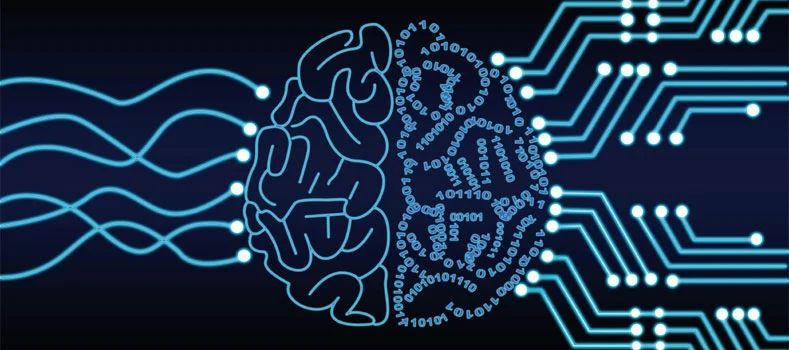
\includegraphics[width=.7\linewidth]{frontpage2}
            
        \Large
        Università degli Studi di Milano
        \\
        Milan\\
        12/04/2020
            
    \end{center}
\end{titlepage}


\newpage

\tableofcontents
\newpage

\subfile{lectures/lecture1}


\newpage
\subfile{lectures/lecture2}

\newpage
\subfile{lectures/lecture3}

\newpage
\subfile{lectures/lecture4}


\newpage
\subfile{lectures/lecture5}


\newpage
\subfile{lectures/lecture6}


\newpage
\subfile{lectures/lecture7}


\newpage
\subfile{lectures/lecture8}


\newpage
\subfile{lectures/lecture9}


\newpage
\subfile{lectures/lecture10}

\newpage
\bibliographystyle{abbrv}
\bibliography{main}

\end{document}
%This is never printed